\documentclass[]{article}
\setlength{\parskip=0.7}{\baselineskip}
\setlength{\parindent}{0pt}

\usepackage{times}
\usepackage{fullpage}

\usepackage{epsfig}
\usepackage{subfigure}

\usepackage{listings}
\usepackage{siunitx}
\usepackage[super]{nth}

\usepackage[sharp]{easylist}

\usepackage{xcolor}

\definecolor{NavyBlue}{cmyk}{0.94,0.54,0,0.5}
\definecolor{BrickRed}{cmyk}{0.16,0.89,0.61,0.2}
\usepackage{url}
\usepackage{breakurl}

\usepackage[
        colorlinks=true,
        urlcolor=NavyBlue, 
        linkcolor=NavyBlue, 
        bookmarksopen=true]{hyperref}
\hypersetup{
    colorlinks,citecolor=NavyBlue,
    linkcolor={red!50!black},
    urlcolor={blue!90!black}
}


\newcommand{\us}{$\mu$s }
\newcommand{\subtopic}[1]{\vspace{1.5pt} \noindent \textbf{#1}}

\definecolor{notecolor}{rgb}{0.75,0,0} % A darker red
\newcommand{\todo}[1]{\textcolor{notecolor}{\textbf{TODO: #1}}}
\newcommand{\hl}[1]{\textcolor{notecolor}{#1}}
\newcommand{\fixit}[2][]{\textcolor{notecolor}{%
     \ifthenelse{\isempty{#1}}{\textbf{[Fixit: %
         #2]}}{\textbf{#2\footnote{\textcolor{notecolor}{Fixit: #1}}}}}}
\newenvironment{highlight}{\par\color{notecolor}}{\par}





\begin{document}

\title{Kawkab: A Distributed Filesystem for Fast Data}
%\author{Sajjad Rizvi, Bernard Wong}
\maketitle

\section{Introduction} Kawkab is a distributed filsesystem developed to
efficiently manage large amounts of streaming data.

\section{Architecture} 

\begin{figure}[t]
    \centering
    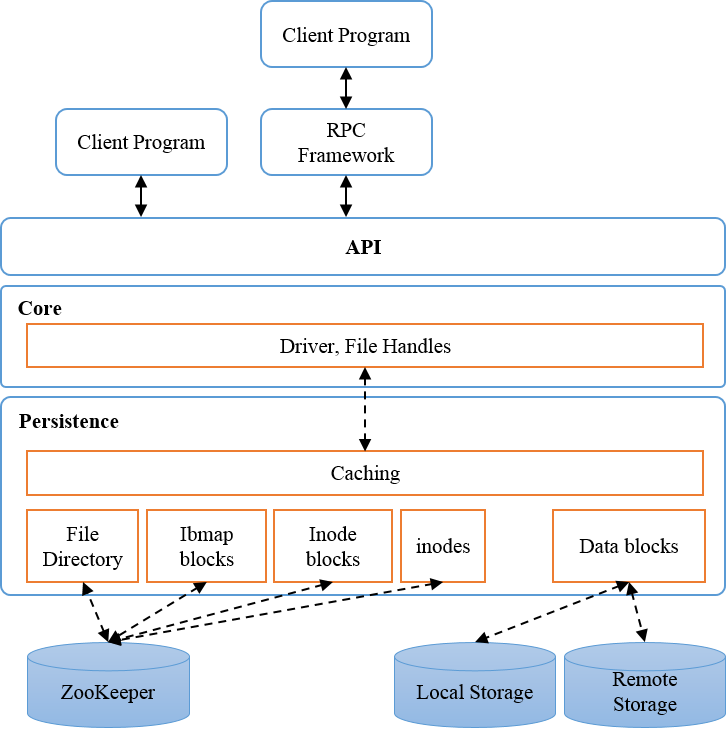
\includegraphics[width=0.5\columnwidth]{{figures/architecture.png}}
    \caption{Kawkab single node architecture.}
   \label{fig:architecture}
\end{figure}

Kawkab mainly follows the design approach of a standard
Unix filesystem. The reasons to follow the Unix filesystem is to control the
memory usage of the system and make the system memory efficient.

The system is divided in three layers: API layer, core, and persistence.
Clients interact with the API layer directly or using an RPC service.  API
provides functions to open, close, read, and write files through the core
layer.

The core layer controls the metadata of the whole system. It mainly consists of
four structures: a file directory, an index node bitmap, index nodes, and data
blocks. Only the data blocks contain the actual data of a file. The other
structures comprise the metadata of the filesystem.

\subsection{Storage Space Design}

\begin{figure}[t]
    \centering
    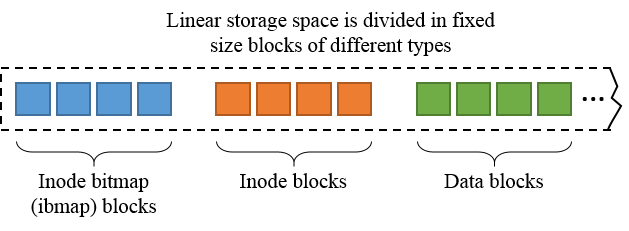
\includegraphics[width=0.5\columnwidth]{{figures/linear-space.png}}
    \caption{Filesystem is designed as a very large storage space organized in fixed size blocks.}
   \label{fig:storage-space}
\end{figure}

\begin{figure}[t]
    \centering
    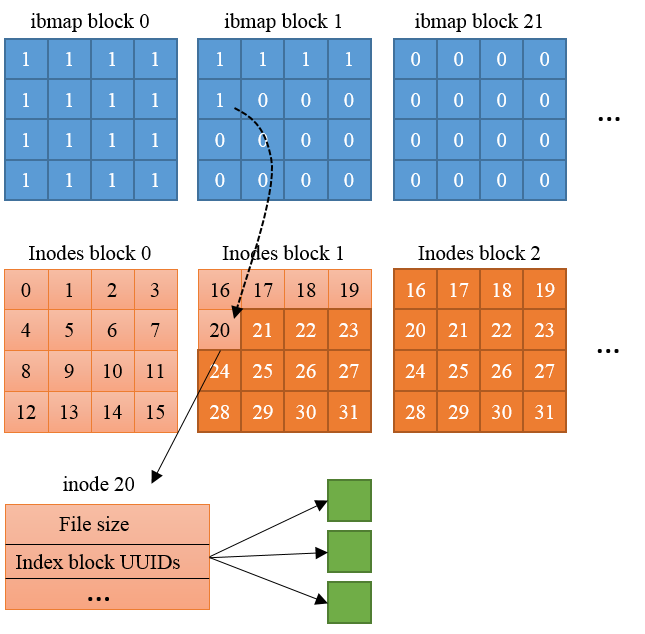
\includegraphics[width=0.5\columnwidth]{{figures/blocks-layout.png}}
    \caption{Layout of different types of blocks.}
   \label{fig:blocks-layout}
\end{figure}



The system is designed such that the files are stored in a very large linear
storage space. The storage space is a collection of fixed size blocks $\{B_1,
B_2, \ldots, B_N\}$.  Each block has a unique ID (UUID), and the blocks are
persistently stored as files on the local storage devices (HDDs, SSDs) and the
cloud, e.g., Amazon EB3 and S3.

The blocks in the storage space are of three types: index node bitmap blocks,
index-node blocks, and data blocks.

\subtopic{Data blocks:} The data blocks contains the actual data belonging to
the files in the system. However, to associate the blocks with a file, the
blocks are indexed using a structure called \textit{index node} or
\textit{inode}. Thus, a file in Kawkab consists of an inode and a collection of
data blocks. The inode, which is further explained in the section~\ref{},
contains the metadata of the file and the IDs of the data blocks belonging
to the file. 

An inode is uniquely referred through a number called \textit{inumber}.
Moreover, an inode is a fixed size structure, and it is stored in an
\textit{index-node block} of our linear storage device.

\subtopic{Index-nodes blocks:} An index-nodes block, or \textit{inode block},
is a fixed size block that contains a predefined number of \textit{inodes}.
%The maximum number of inode blocks in the system controls the maximum number
%of files supported in the system because the filesystem has a fixed number of
%inode blocks.  As the filesystem has fixed number of inode blocks, which also
%controls the number of files supported by the system.
As each inode has a fixed size $S_I$ bytes, an inode block $B$ contains $N =
S_{B} / S_I$ number of inodes, where $S_B$ is the size of an inodes block.
Thus, the inode number $x$ is located in the inode block number $ x / N$. In
this way, given an inode number, Kawkab can calculate the inode block that
contains the inode, and the index of the inode in the block.

When a file is created, the file is assigned a unique inumber, which
is the first available inode number in the system. To achieve that, the
system keeps track of the inumbers already assigned using a bitmap
called \textit{inode bitmap} or \textit{ibmap}. The ibmap is stored in
the blocks of type "inode bitmap block".


\subtopic{Inode Bitmap Blocks:} An inode bitmap block, or ibmap block,
is a fixed size block that contains part of the ibmap. 
Each bit at index $i$ in the ibmap indicates whether the inode of inumber $i$ 
is already used or not. 

When a new file is created, Kawkab scans the ibmap to find the first unused 
inumber and assigns that inumber to the inode associated with the file. Moreover,
Kawkab sets the bit in the bitmap that is associated with the inumber.
When a file is deleted, Kawkab clears the bit in the ibmap, which allows
Kawkab to reuse the inode and the inumber for the next new file.


\subsection{File Directory} Kawkab filesystem contains a file directory that
defines the namespace of the system.
%The file directory keeps track of the existing files in the system and the way
%to access the files.
Each file in the system has a unique name and a unique inode number.  The file
directory is a simple collection of $\langle$ file name, inode number $\rangle$
pairs that maps a file name to an inode number.  The clients refer to a file
using the file name whereas the system access the files through the inode
numbers. 

The file directory is the only structure that keeps the mapping of the file
names and the inode numbers. Therefore, the file directory is made persistent
and consistent through a key value store such as LMDB, Berkley DB, or LevelDB.

\subtopic{File Namespace:} Kawkab has a flat namespace. Kawkab does not maintain
directory hierarchies. However, a user can use any file name.



\subsection{Index Node} An index node, called \textit{inode}, is the main
structure that keeps track of the file metadata and IDs of the data
blocks associated with the file. An inode is a fixed size structure that
consists of the following parts:

\begin{enumerate}
  \item \subtopic{File Metadata:} The file metadata consists of information
        about the file such as file creation time, last access time, file
        rights, and file size.

	\item \subtopic{First $N$ Data Blocks:} An inode contains a fixed number
$N$ of the IDs of the first $N$ data blocks associated with the file.
These data blocks are directly accessible from the inode and requires
only one step lookup in the inode.
%An inode keeps the reference of the first $N$ data blocks of the file. 
The number $N$ is kept small to optimize for the memory space and the file
access for smaller files. 

  \item \subtopic{Indirect Block:} 
An inode contains the ID of one indirect block, where an indirect block is
special data block that only consists of the IDs of the data blocks associated
with the file. Thus, an indirect block is level-1 index into the file.
As the size of each block is fixed, an indirect block contains the
IDs of a fixed number of data blocks in a file. These data blocks 
range from $N+1$ to $M$ where $M$ is the number of IDs stored in the
direct block.

  \item \subtopic{Double and Triple Indirect Block:}
An inode has one double and one triple indirect block. A double indirect block is a two
level index, i.e., a double indirect block is the ID of a special data block that contains
the IDs of indirect blocks. Similarly, a triple indirect block contains the IDs of the
double indirect blocks. These indexing levels are sufficient to support the maximum 
file size in Kawkab, which is $2^{63}-1$ bytes.

\end{enumerate}

\subsection{Data Blocks} Kawkab has fixed size data blocks. Each data block has
a unique ID, generated as a UUID.  Each block is persistently stored as a file
in the persistent storage of the system, e.g., local or remote disks, EB3, or
S3.  The name of the persistent file is extracted from the UUID: the UUID is
converted to an ASCII character string using Base64 encoding.  The ASCII name
is then converted into a file path such that each two characters in the ASCII
representation of the UUID become a directory name in the persistent storage.
For example, a UUID \texttt{ABCDEFGH} is stored as a file
\texttt{/storage/datablocks/AB/CD/EF/GH}.


\subsection{Persistence Layer}
\hl{Note: This section is incomplete.}

The persistence layer in Kawkab keeps track of the location of each file in the system.
All the blocks are stored and retrieved from the persistence layer using the UUIDs
of the blocks.

The persistence layer has a caching sub-module. The caching module acts as an
LRU cache and controls the memory of one machine.


\subsection{Block Metadata} In order to achieve faster data access, each block
has an associated metadata that is stored along with the block's UUID. The
metadata includes: first append time, last append time, and the additional
data boundaries that allow fine grained indexing within a data block.

\subsection{Data Access and Indexing}
\hl{Note: This section is incomplete.}

Kawkab is an append-only system. Each append is performed at the end of the file.
However, a file can be read from any location. When a client opens a file,
it is returned a FileHandle. The FileHandle contains a read pointer that indicates
the current position in the file from where the data will be read. The read
pointer can be moved to any position in the file using any of the following
ways: 

\begin{enumerate}
  \item Move to an absolute byte offset in the file.
  \item Give a timestamp T:
  \begin{itemize}
    \item Move to the first byte of the closest block that has the append time equal to
          or \textit{before} T.
    \item Move to the first byte of the closest block that has the append time equal to
          or \textit{after} T.
  \end{itemize}
\end{enumerate}

In order to find the data block that contains the given byte or timestamp, Kawkab
performs binary search over the index in the inode.

%  - How data is indexed
% - How data is retrieved given a byte offset
 % - How data is retrieved given a timestamp

\subsection{Atomic Appends and Reading Unfinished Block}

\section{Comparison with Existing Systems}

\begin{easylist}[itemize]

 # Comparison with Alluxio

 # Comparison with Succinct

 # Comparison with HDFS and similar systems

\end{easylist}

\begin{figure}[t]
    \centering
    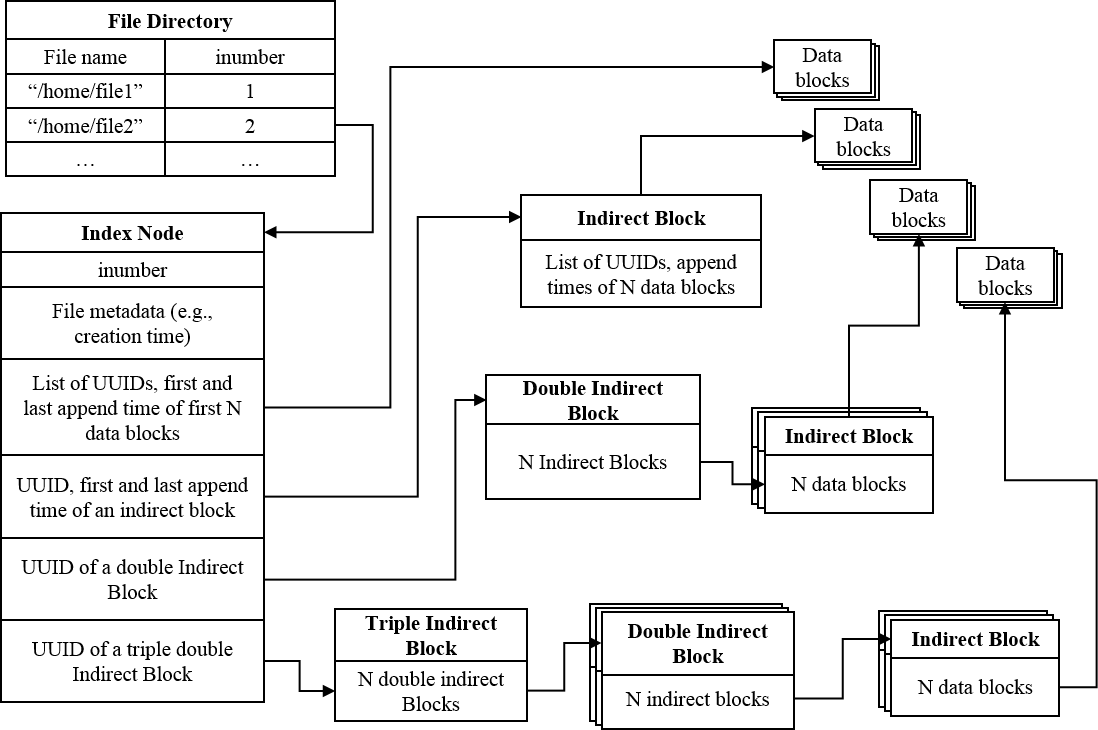
\includegraphics[width=0.9\columnwidth]{{figures/file-index-design.png}}
    \caption{File directory and file index.}
   \label{fig:data-structures}
\end{figure}



\end{document}
